% TODO: Cleanup scalebox.
\documentclass[tikz]{standalone}
\usepackage{pgfplots}
\pgfplotsset{compat=1.15}
\usepackage{mathrsfs}
\usetikzlibrary{arrows,calc}
\usepackage{tkz-euclide}

\pagestyle{empty}

\definecolor{AngleClr}{rgb}{0,0.39215686274509803,0}
\definecolor{ShapeClr}{rgb}{0.6,0.2,0}

\begin{document}

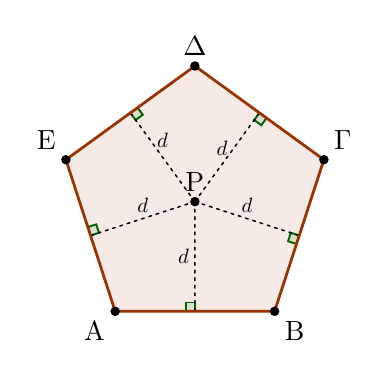
\begin{tikzpicture}[scale=.75]
\tkzSetUpLine[line width=1pt,color=black]
\tkzSetUpPoint[fill=black]

\tkzDefPoints{0/0/P0,2.7/0/P1,1.755/0.81/P}
\tkzDefRegPolygon[side,sides=5](P0,P1)

\tkzDefTriangleCenter[circum](P1,P2,P3) \tkzGetPoint{P}

\tkzDefPointBy[projection = onto P1--P2](P) \tkzGetPoint{D1}
\tkzDefPointBy[projection = onto P2--P3](P) \tkzGetPoint{D2}
\tkzDefPointBy[projection = onto P3--P4](P) \tkzGetPoint{D3}
\tkzDefPointBy[projection = onto P4--P5](P) \tkzGetPoint{D4}
\tkzDefPointBy[projection = onto P5--P1](P) \tkzGetPoint{D5}


\tkzFillPolygon[fill=ShapeClr,fill opacity=0.1](P1,P2,P3,P4,P5)

\tkzMarkRightAngles[line width=0.7pt, size=.15,color=AngleClr,fill=AngleClr,fill opacity=0.1](P,D1,P1 P,D2,P2 P,D3,P3 P,D4,P4 P,D5,P5)

\tkzDrawSegments[line width=0.55pt,color=black,dashed,dash pattern=on 1pt off 1.75pt](P,D1 P,D2 P,D3 P,D4 P,D5)

\tkzDrawPolygon[color=ShapeClr](P1,P2,P3,P4,P5)
\tkzDrawPoints[size=3](P1,P2,P3,P4,P5,P)
\tkzLabelPoint[below left](P1){$\rm A$}
\tkzLabelPoint[below right](P2){$\rm B$}
\tkzLabelPoint[above right](P3){$\rm \Gamma$};
\tkzLabelPoint[above](P4){$\rm \Delta$};
\tkzLabelPoint[above left](P5){$\rm E$};
\tkzLabelPoint[above](P){$\rm P$};

\tkzLabelSegment[left=-1.5pt](P,D1){\scalebox{0.75}{$d$}}
\tkzLabelSegment[above=-1.5pt](P,D2){\scalebox{0.75}{$d$}}
\tkzLabelSegment[left=-1.5pt,pos=0.6](P,D3){\scalebox{0.75}{$d$}}
\tkzLabelSegment[above](P,D4){\scalebox{0.75}{$d$}}
\tkzLabelSegment[above=-1.5pt](P,D5){\scalebox{0.75}{$d$}}

\end{tikzpicture}

\end{document}
